  \section{Symulacje numeryczne}
  
  
  \subsection{Oprogramowanie}

  Do oprogramowania symulacji wybrałem język Java, jako oferujący dobrą wydajność w obliczeniach numerycznych, z dojrzałym ekosystemem narzędzi i bibliotek oraz wieloplatformowy. Oskryptowanie zestawów symulacji (''przemiatanie'' po parametrach, wiele powtórzeń dla uśrednienia wyników) wykonałem w języku Groovy.
  
  Kod źródłowy jest dostępny jako open-source w serwisie GitHub pod adresem http://github.com/tomash/fhneurotic .

  \subsubsection{Obliczanie widma mocy}

  Widmo mocy obliczane było z użyciem biblioteki JTransforms, przy pomocy szybkiej transformaty Fouriera (FFT). Ponieważ dane wejściowe, tj. wartości potencjału $v$ w zależności od czasu, były rzeczywiste, zastosowana została jednowymiarowa szybka transformata Fouriera dla danych rzeczywistych:

  \begin{equation}
    F_k = \sum\limits^{N-1}_{n=0} v_n e^{-i2\pi \frac{k}{N} n} ,
  \end{equation}

  z zastrzeżeniem że algorytm liczył połowę elementów rzeczywistej transformaty, ponieważ druga połowa spełniała warunek symetrii

  \begin{equation}
    F_{N-k} = F^{*}_{k} \quad .
  \end{equation}

  Biblioteka JTransforms do obliczenia FFT z danych rzeczywistych stosuje algorytmy Split-Radix oraz Mixed-Radix. Dla optymalizacji obliczania FFT, liczba kroków symulacji (wartości $v$ poddawanych transformacie) jest potęgą 2.

  Widmo mocy było obliczane jako kwadrat modułu transformaty Fouriera:

  \begin{equation}
    S_k = |F_k|^2
  \end{equation}

  $F_k$, a więc i tym samym $S_k$, nie były normalizowane dalszych w obliczeniach.

  \subsubsection{Obliczanie Signal-to-Noise Ratio}

  Stosunek sygnału do szumu w widmie mocy obliczałem poprzez podzielenie najwyższej wartości widma (tj. piku głównego) przez średnią 10 wartości sąsiadujących (5 niższych, 5 wyższych).

  \begin{equation}
    SNR = \frac{S_i}{\frac{1}{10} \left ( \sum\limits^{i-1}_{j=i-5} S_j + \sum\limits^{i+5}_{j=i+1} S_j \right )} ,
  \end{equation}

  gdzie $i$ jest indeksem odpowiadającym częstotliwości wymuszenia periodycznego $\beta$.

  \subsection{Parametry symulacji}
  \label{sec:parametry}

  Punktem wyjścia do symulacji była praca A. Longtin \cite{longtin}, włączając w to znalezione przez niego optymalne zestawy parametrów pozwalające zaobserwować rezonans stochastyczny w neuronie FHN. Parametry symulacji, jeśli nie podano inaczej, są następujące:

  \begin{itemize}
    \item krok czasowy $\Delta t = 1/256 [s]$
    \item czas korelacji szumu $t_c = 0.01 [s]$
    \item okres sygnału periodycznego $T=1.0 [s]$ (częstotliwość $f=T^{-1}=1.0 [\frac{1}{s}]$), tym samym częstość $\beta = \frac{2 \pi}{T} = 2 \pi [\frac{1}{s}] $
    \item skalowanie czasu dla $v$ (''szybkiej'' zmiennej) $\epsilon = 0.005$
    \item amplituda sygnału periodycznego $r=0.08$
    \item stała relaksacji $b=0.12$
    \item $a$ z równania (\ref{eq:v}) $a=0.5$
  \end{itemize}

  \subsection{Pojedynczy Neuron}

  \subsubsection{Metodologia}
  
  Przed przystąpieniem do rozwiązywania układów wieloneuronowych rozpocząłem symulacje od zbadania pojedynczego neuronu, jak opisywany w pracy A. Longtin \cite{longtin}. Dzięki temu mogłem sprawdzić zarówno poprawność własnego oprogramowania, jak i model oraz zestaw parametrów opisane w wyżej wymienionej publikacji.
  
  Stochastyczne równania różniczkowe składające się na szum Ornsteina-Uhlenbecka całkowałem według metody opisanej w pracy Mannella, Palleschi \cite{mannella}. Po rozwiązaniu przedstawionego tam równania, szum $\eta (t)$ obliczany był następująco:

  \begin{equation} \label{eq:deta:final}
    \Delta \eta(t) = \Delta t(\lambda \xi_1(t) - \lambda \eta(t)) + \lambda \xi_2(t) \sqrt{\Delta t}
  \end{equation}

  \begin{equation} \label{eq:eta:final}
    \eta(t) = \eta(t-\Delta t) + \Delta \eta(t)
  \end{equation}

  Gdzie $\xi_1(t)$, $\xi_2(t)$ to dwa niezależne, białe szumy gaussowskie w chwili t :

  \begin{equation} \label{eq:eta:gauss}
    \langle \xi_i(t) \xi_j(s) \rangle\ = 2 \delta_{ij} \delta (t-s) .
  \end{equation}

  Równania różniczkowe składające się na dynamikę neuronu FHN całkowałem metodą Eulera:

  \begin{equation} \label{eq:discrete1:deltav}
    \Delta v = \frac{1}{\epsilon} \Delta t [v(v-a)(1-v)- \omega  + \eta(t) + sv_{ext}(t)]
  \end{equation}

  \begin{equation} \label{eq:discrete1:v}
    v(t) = v(t-\Delta t) + \Delta v(t)
  \end{equation}

  \begin{equation} \label{eq:discrete1:deltaw}
    \Delta \omega = \Delta t [v - d \cdot \omega - [b + r sin(\beta t + \phi)]]
  \end{equation}

  \begin{equation} \label{eq:discrete1:w}
    \omega(t) = \omega(t-\Delta t) + \Delta \omega(t)
  \end{equation}


  \subsubsection{Symulacja pojedynczego neuronu}
  
  Wyniki symulacji dla pojedynczego neuronu, z zestawem parametrów jak w \cite{longtin}, przedstawiają rysunki \ref{graphics:sym1v} (przebieg czasowy) i \ref{graphics:sym1fft} (widmo mocy).

  
  \begin{figure}
    \begin{center}
      \begin{tabular}{cc}
        \resizebox{100mm}{!}{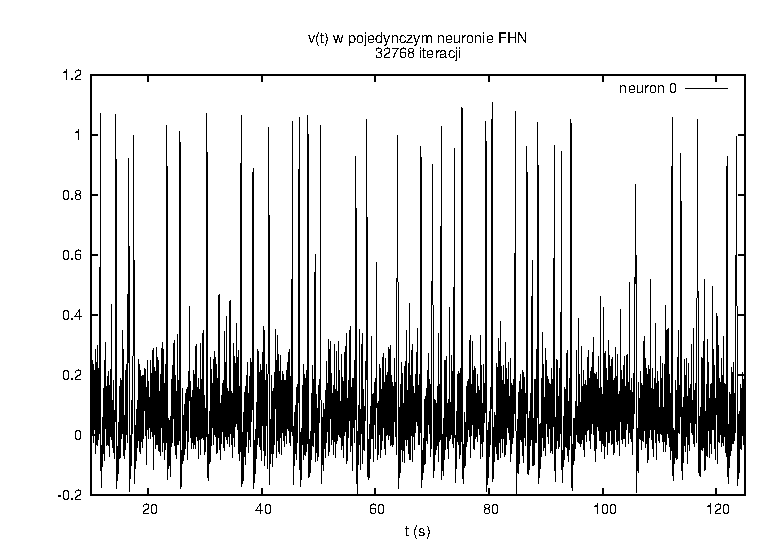
\includegraphics[width=140mm]{images/1neuron/1}} \\
        \resizebox{100mm}{!}{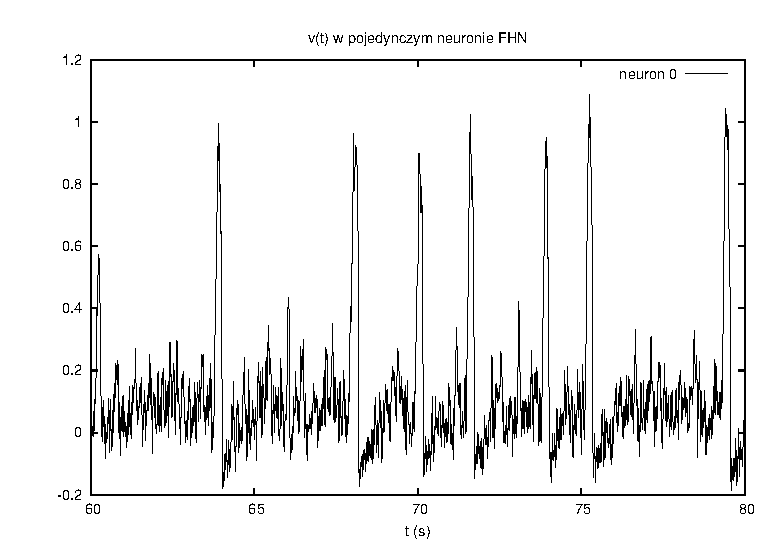
\includegraphics[width=140mm]{images/1neuron/2}} \\
      \end{tabular}
      \caption{Odtworzenie wyników Longtina z pracy \cite{longtin}. 32768 kroków iteracji, $D=1 \cdot 10^{-5}$, pozostałe parametry jak w rozdziale \ref{sec:parametry}.}
      \label{graphics:sym1v}
    \end{center}
  \end{figure}

  Jest to przebieg zgodny z zaobserwowanym w pracy A. Longtin.

  \begin{figure}
    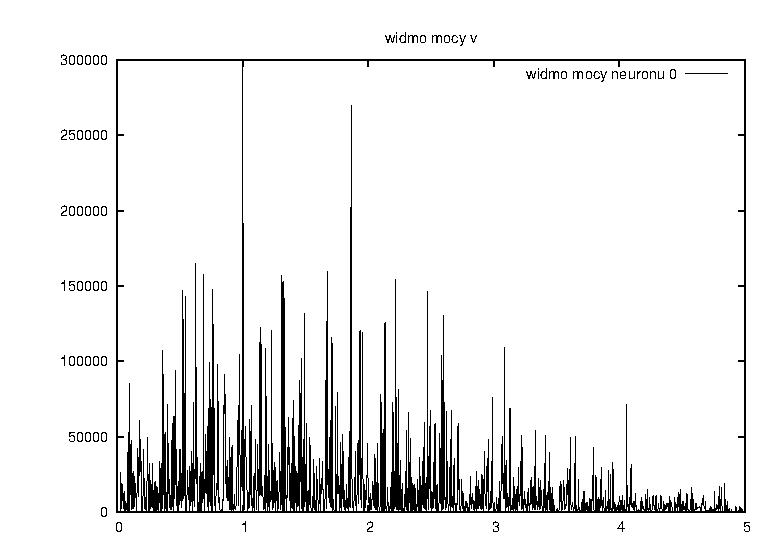
\includegraphics[width=140mm]{images/1neuron/3}
    \caption{Odtworzenie wyników Longtina z pracy \cite{longtin}: widmo mocy. Widać wyraźne piki dla częstotliwości podstawowej sygnału periodycznego $f=1.0$ i jej wielokrotności. Dla piku głównego SNR = 8.26.}
    \label{graphics:sym1fft}
  \end{figure}

  
  \subsection{Układy neuronów bez opóźnienia}
  \label{sec:uklad_bez_opoznienia}

  \subsubsection{Metodologia}
  
  Następnym krokiem pracy było połączenie neuronów (początkowo dwóch) w łańcuch, bez opóźnień w transmisji sygnałów.

  Jak już wspomniano w rozdziale \ref{sec:zagadnienia_badane}, topologia połączeń pomiędzy neuronami jest taka, że potencjały przekazywane są ''w jedną stronę'', tzn. sygnał z neuronu $i$ jest odbierany przez neuron $i-1$ (neuron o indeksie 0 nie przekazuje swojego sygnału dalej, neuron o najwyższym indeksie nie odbiera sygnału od sąsiada). Wraz z zerowymi opóźnieniami w transmicji, założenia te prowadzą do następującej postaci równania (\ref{eq:vext1}):

  \begin{equation} \label{eq:vext2}
    v_{i ext}(t) = \widetilde{v_{i+1}}(t)
  \end{equation}

  Neurony w układzie działały według równań (\ref{eq:v2}, \ref{eq:w2}) zaproponowanych w rozdziale \ref{sec:przestrzennie_rozciagly_fhn}, bez opóźnienia (czyli $\tau_{i,n} = 0$).

  Ważnym elementem tego etapu badań było dobranie nowej wartości skalowania szumu $D$. Dotychczasowa wartość, czyli $D=1 \cdot 10^{-5}$, powodowała maksymalizację SNR w pojedynczym neuronie, ale w macierzach neuronów powoduje tłumienie wpływu sygnałów odebranych od połączonych neuronów (przesterowanie).

  Po wielu symulacjach z różnymi zakresami parametrów (patrz też wykres \ref{fig:graphics:snr_c_d_3d}) ustaliłem wartość $D$ w okolicach $D=5 \cdot 10^{-6}$ jako pozwalającą zaobserwować SR w pojedynczym neuronie jak i obserwować wyraźne zwiększanie SNR w wyniku odbierania sygnału od połączonych neuronów. Dla potwierdzenia tej hipotezy dalsze symulacje prowadzone były dla wartości $D$ w zakresie od $D=1 \cdot 10^{-6}$ do $D=2 \cdot 10^{-5}$. 

  Ważna jest też czułość na sygnał odebrany od połączonego neuronu. Modelu FHN ma dynamikę bardzo podatną na zmiany parametrów, nawet w wąskich zakresach. W pracy Longtina dobrano optymalną amplitudę sygnału periodycznego $r=0.08$. Jest to wartość bardzo wysoka, gwarantująca silnie periodyczne zachowanie pojedynczego neuronu (dla wartości szumu z zakresu $5 \cdot 10^{-6} - 5 \cdot 10^{-5}$), podczas kiedy jest ono dość periodyczne już dla $r=0.05$. Suma amplitudy sygnału periodycznego i amplitudy sygnału odbieranego od sąsiednich neuronów nie powinna przekraczać maksymalnej użytecznej amplitudy sygnału periodycznego dla pojedynczego neuronu $r_{max}=0.08$.
  
  Po wielu próbach wybrano amplitudę $r=0.05$ i stałą sprzężenia $s=0.02$, jako pozwalające uzyskać wyraźny wpływ połączonych neuronów, a jednocześnie zwiększać SNR w kolejnych neuronach łańcucha bez wysycenia (osiągnięcia maksimum SNR i przesterowania kolejnych neuronów) na drugim-trzecim neuronie.

  Powyższe rozważania oparte są o symulacje i analizy układu dwóch neuronów (transmisja sygnału od neuronu $i=1$ do neuronu $i=0$), służyły one wyłącznie dobraniu optymalnego zakresu parametrów dla dalszych symulacji bardziej rozbudowanych układów.

  \subsubsection{Łańcuch 9 neuronów bez różnicy faz}
  \label{sec:lancuch_9_bez_roznicy_faz}

  Po znalezieniu optymalnego zakresu parametrów dla układu wieloneuronowego, kolejnym etapem pracy było zbadanie łańcucha $N=9$ neuronów.

  Zbudowany według powyższych założeń łańcuch 9 neuronów był symulowany numerycznie, najpierw bez rozciągłości przestrzennej układu, czyli $\phi_i = 0 \quad, i=0...,(N-1) $, oraz bez opóźnień, czyli $\tau_{i,i+1}=0$.

  Wynik symulacji tak zbudowanego układu przedstawia rysunek \ref{fig:graphics:sim:2011_12_07_01}, z bardziej czytelnym przecięciem płaszczyznami $i=0$ i $i=8$ na rysunku \ref{fig:graphics:sim:2011_12_07_02}.

  \begin{figure}
    \includegraphics[width=140mm]{images/9neuron/2011_12_07_01}
    \caption{Układ 9 neuronów bez opóźnienia, bez róznic fazowych. Widać wyraźny wzrost SNR zgodnie z ''kierunkiem'' przekazywania sygnału. $r=0.05$, $s=0.02$, SNR obliczony na podstawie nienormalizowanego widma mocy. 65536 ($2^{16}$) kroków iteracji (256 okresów) dla każdego zestawu parametrów. Wartości SNR uśrednione, po 20 pełnych symulacji dla każdej wartości $D$.}
    \label{fig:graphics:sim:2011_12_07_01}
  \end{figure}

  \begin{figure}
    \includegraphics[width=140mm]{images/9neuron/2011_12_07_02}
    \caption{Przecięcie wyników z rysunku \ref{fig:graphics:sim:2011_12_07_01} płaszczyznami $n=0$ (SNR w neuronie odbierającym sygnał na końcu) i $n=8$ (SNR w neuronie nieodbierającym sygnału)}
    \label{fig:graphics:sim:2011_12_07_02}
  \end{figure}

  Zaobserwowane przebiegi czasowe były zgodne ze spodziewanym analitycznie wynikiem: z każdym kolejnym neuronem w łańcuchu następował wzrost SNR (do wartości granicznej około 200, stwierdzonej podczas symulacji pojedynczych neuronów) ze względu na wzrost prawdopodobieństwa wzbudzenia w przypadku wzbudzenia neuronu sąsiedniego. Zaobserwowano więc zjawisko analogiczne do AESR, jak opisane w rozdziale \ref{sec:wzmocnienie_przez_sprzezenie}.

  \subsubsection{Łańcuch 9 neuronów z różnicą faz}

  Następnym krokiem było wprowadzenie do układu rozciągłości przestrzennej, czyli uwzględnienie różnic w fazach sygnału periodycznego odbieranego przez poszczególne neurony, na tym etapie bez opóźnień transmisji. Aby zmaksymalizować efekt antysynchronizacji, wybrano różnicę faz pomiędzy sąsiadującymi rezonatorami równą $\Delta \phi_{i,i+1} = \phi_{i} - \phi_{i+1} = \pi $.

  Badany układ opisywany był więc równaniami (\ref{eq:v2}, \ref{eq:w2}) z $\phi_i = -\pi \cdot i$ i potencjałem odbieranym od sąsiadów, danym równaniem (\ref{eq:vext2}).

  Oczekiwanym skutkiem było gwałtowne obniżenie SNR we wszystkich neuronach z wyjątkiem ostatniego (jako że nie odbiera on sygnału od sąsiadujących neuronów). Wyniki przedstawia rysunek \ref{fig:graphics:sim:2011_12_06_01}.

  SNR w neuronach odbierających sygnały ($i=0...(N-2)$) ulega obniżeniu, ponieważ sygnały periodyczne w neuronach $i$ i $i+1$ są przesunięte w fazie o pół okresu. W chwili gdy sygnał periodyczny w neuronie $i$ ma wartość minimalną, co powinno prowadzić do obniżenia jego aktywności (faza relaksacji, niskie prawdopodobieństwo emisji potencjału czynnościowego), sygnał periodyczny w neuronie $i+1$ ma wartość maksymalną, a zatem z dużym prawdopodobieństwem neuron ten jest aktywny i w trakcie emisji szpilki potencjału. Emitowany potencjał dociera do neuronu $i$ bez opóźnienia, zwiększając prawdopodobieństwo emisji przez niego szpilki potencjału czynnościowego. Wpływ sygnału odbieranego przez neuron $i$ (od neuronu $i+1$) na aktywność tego neuronu jest tym samym przeciwny do wpływu sygnału periodycznego, wskutek czego prawdopodobieństwo pobudzenia neuronu staje się słabo zależne od czasu. Skutkuje to obniżeniem SNR w porównaniu do neuronu niesprzężonego, z takim samym zestawem pozostałych parametrów (patrz SNR w neuronie $i=8$ w tej symulacji).
  Jest to przykład negatywnego wpływu przesunięć fazowych sygnału periodycznego w układzie oddziałujących rezonatorów stochastycznych, zjawiska przeciwnego do AESR. Analogiczne zjawisko było opisane w pracy \cite{ijmpb_14_8}.

  \begin{figure}
    \includegraphics[width=140mm]{images/9neuron/2011_12_06_01}
    \caption{Układ 9 neuronów bez opóźnienia, z różnicą faz $\Delta \phi_{i,i+1} = \pi $. Widać, że dla neuronów które odbierały sygnał od sąsiada SNR utrzymuje się na bardzo niskim poziomie, o wiele niższym od neuronu nieodbierającego sygnału (neuron ósmy). Parametry jak w symulacjach przedstawionych na rys. \ref{fig:graphics:sim:2011_12_07_01}. Dla czytelności wykres został obrócony (neuron $i=0$ na ''dole'') względem pozostałych wykresów trójwymiarowych dla łańcucha 9 neuronów.}
    \label{fig:graphics:sim:2011_12_06_01}
  \end{figure}


  \subsection{Układy neuronów z opóźnieniem}

  Aby rozciągłe przestrzennie układy połączonych neuronów doprowadzić do zwiększenia synchronizacji (i tym samym podwyższyć SNR względem pojedynczego neuronu), zamiast jej zmniejszenia, wprowadzone zostało opóźnienie w transmisji, celem kompensacji różnicy faz odbieranego przez poszczególne neurony sygnału periodycznego.

  \subsubsection{Metodologia}
  
  Do układu opisanego powyżej dodałem opóźnienie w przekazywaniu sygnałów, w sposób opisany w rozdziale ~\ref{sec:przesuniecie_fazy}. Łańcuch został zbudowany jak w rozdziale \ref{sec:uklad_bez_opoznienia}, a następnie wprowadzono opóźnienie. Pomiędzy każdą parą sąsiadujących neuronów opóźnienie jest jednakowe dla wszystkich par i wynosi $\tau$. Te założenia prowadzą do następującej postaci równań (\ref{eq:v2}, \ref{eq:w2}) i równania (\ref{eq:vext2}):

  \begin{equation}
    \epsilon \frac{dv_i}{dt} = v_i(v_i-a)(1-v_i)- \omega  + \eta_i(t) + sv_{iext}(t)
  \end{equation}

  \begin{equation}
    \frac{d \omega_i}{dt} = v_i - d \cdot \omega_i - [b + r sin(\beta t + \phi_i)]
  \end{equation}

  \begin{equation}
    v_{i ext}(t) = \widetilde{v_{i+1}}(t-\tau)
  \end{equation}

  Wykonane zostały symulacje łańcuchów złożonych z 2. i 9. rezonatorów.
  
  \subsubsection{Łańcuch 2 neuronów}

  Pierwszym krokiem w badaniu macierzy neuronów z opóźnieniem uczyniłem zbadanie macierzy dwuelementowej, celem znalezienia zależności pomiędzy podstawowymi parametrami symulacji.

  Przez $c$ oznaczyłem opóźnienie transmisji, jako wielokrotność okresu sygnału periodycznego $\tau = c T$. Przesunięcie fazowe sygnału periodycznego pomiędzy sąsiednimi neuronami wynosiło pół okresu $\Delta \phi_{i,i+1} = \pi$ (czyli $\phi_i = -i \cdot \pi$).
  Znaleziona i przedstawiona na rysunku \ref{fig:graphics:snr_c_d_3d} zależność SNR od $c$ oraz $D$ posiada bardzo wyraźną ''grań'' dla $c=0.5$, co potwierdza oczekiwania: maksymalizację SNR można osiągnąć poprzez kompensację przesunięcia fazowego (rozciągłości przestrzennej) odpowiednio dobranym opóźnieniem w transmisji.
  Ze względu na wspólne parametry symulacji, można porównać wyniki uzyskane w symulacjach różnych układów. Wykres na rysunku \ref{fig:graphics:snr_c_d_3d} został przecięty płaszczyzną $c=0.5$ i, na rysunku \ref{fig:graphics:snr_comparison}, porównany z przecięciem wykresu na rysunku \ref{fig:graphics:sim:2011_12_07_01} dla $i=7$ (SNR w pierwszym z odbierających neuronów).

  \begin{figure}
    \includegraphics[width=140mm]{images/2neuron/3d_2}
    \caption{Dwa neurony, SNR w odbierającym neuronie $i=0$, jako zależność od opóźnienia w transmisji c ($\tau = c T$), dla przesunięcia fazowego równego $\Delta \phi_{0,1} = \pi$. Widać wyraźną ''grań'' kiedy c = 0.5. 65536 ($2^{16}$) kroków iteracji (256 okresów) dla każdego zestawu parametrów.}
    \label{fig:graphics:snr_c_d_3d}
  \end{figure}

  \begin{figure}
    \includegraphics[width=140mm]{images/compare/n07}
    \caption{Porównanie SNR neuronu $i=0$ z symulacji przedstawionej na rys. \ref{fig:graphics:snr_c_d_3d} i SNR neuronu $i=7$ z symulacji przedstawionej na rys. \ref{fig:graphics:sim:2011_12_07_01}. 65536 ($2^{16}$) kroków iteracji (256 okresów) dla każdego zestawu parametrów. Wartości i kształt są zbliżone, a różnice (zwłaszcza dla niskich amplitud szumu $D$) wyjaśnialne fluktuacjami SNR wynikającymi ze stochastyczności procesu.}
    \label{fig:graphics:snr_comparison}
  \end{figure}

  Wyniki dla dwóch neuronów potwierdzają hipotezę. Przystąpiłem zatem do symulowania przestrzennie rozciągłego łańcucha 9. neuronów z opóźnieniami.

  \subsubsection{Łańcuch 9 neuronów z opóźnieniem}

  Najpierw zostały zbadane łańcuchy neuronów FHN połączonych tak, aby opóźnienie transmisji kompensowało rozciągłość przestrzenną, czyli $c = \frac{\Delta \phi_{i,i+1}}{2 \pi}$. Takie łańcuchy powinny dawać wyniki zbliżone do układu o tej samej strukturze, ale bez opóźnień i przesunięć fazowych, jak przedstawione w rozdziale \ref{sec:lancuch_9_bez_roznicy_faz}.

  Przyjęto przesunięcie fazowe z warunkiem periodycznym, tzn. dla łańcucha $N=9$ neuronów różnica faz wynosi $\Delta \phi_{i,i+1} = \frac{1}{9} 2 \pi \approx 0.111 \cdot 2 \pi$.
  
  \begin{figure}
    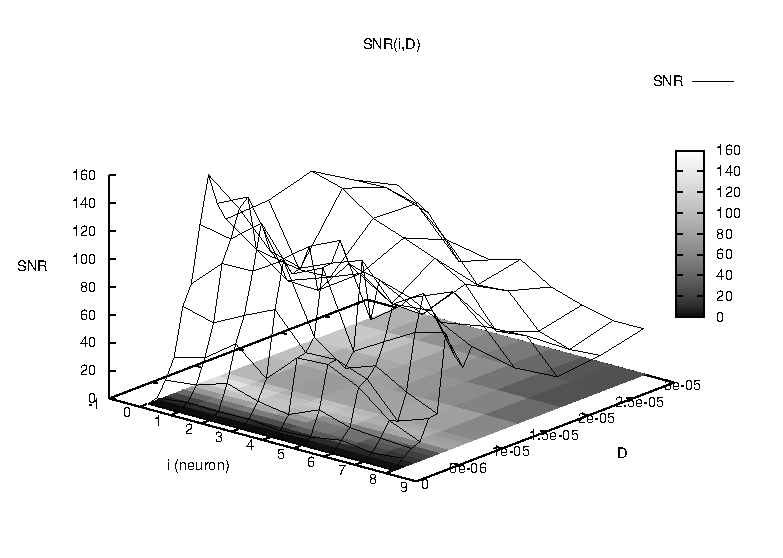
\includegraphics[width=140mm]{images/9neuron/2011_12_07_04}
    \caption{Układ 9 neuronów rozciągły przestrzennie o przesunięciu fazowym $\Delta \phi_{i,i+1} = 0.111 \cdot 2 \pi$ z opóźnieniem transmisji dobranym do kompensowania rozciągłości przestrzennej $c = 0.111 T$. 65536 ($2^{16}$) kroków iteracji (256 okresów). Widać duże podobieństwo (z dokładnością do fluktuacji) z wykresem na rys. \ref{fig:graphics:sim:2011_12_07_01}}
    \label{fig:graphics:sim:2010_12_07_04}
  \end{figure}

  Wyniki, przedstawione na rysunku \ref{fig:graphics:sim:2010_12_07_04}, są zgodne z oczekiwaniami: przestrzennie rozciągły łańcuch neuronów z opóźnieniami transmisji kompensującymi różnice fazowe w istocie zachowuje się jak analogiczny układ pozbawiony opóźnień i różnic fazowych, z dokładnością do fluktuacji SNR wynikających ze stochastyczności równań.

  \subsubsection{Łańcuch 9 neuronów z opóźnieniem i niespójną różnicą faz}

  Rzeczywiste układy przestrzennie rozciągłe nie zawsze zachowują idealne odległości pomiędzy elementami. Czasem odległości ulegają pewnym fluktuacjom, co odpowiednio zmianę fazy odbieranej fali biegnącej.
  Ostatnim badaniem przeprowadzonym w ramach niniejszej pracy było zbadanie czy układ przestrzennie rozciągły z opóźnieniami jest odporny na niewielkie fluktuacje różnicy faz.

  W tym celu do łańcucha 9 neuronów, takiego jak symulowany we wcześniejszych eksperymentach, użyte zostało fluktuowane przesunięcie fazowe $\Delta \psi_{i,i+i}$, liczone na podstawie dotychczas stosowanego $\Delta \phi_{i,i+i}$ pomnożonego przez fluktuację:

  \begin{equation}
    \Delta \psi_{i,i+1} = \Delta \phi_{i,i+1} \cdot \zeta_{i,i+1}
  \end{equation}

  gdzie $\zeta_{i,i+1}$ jest liczbą losową z zakresu $0.9 - 1.1$.

  \begin{figure}
    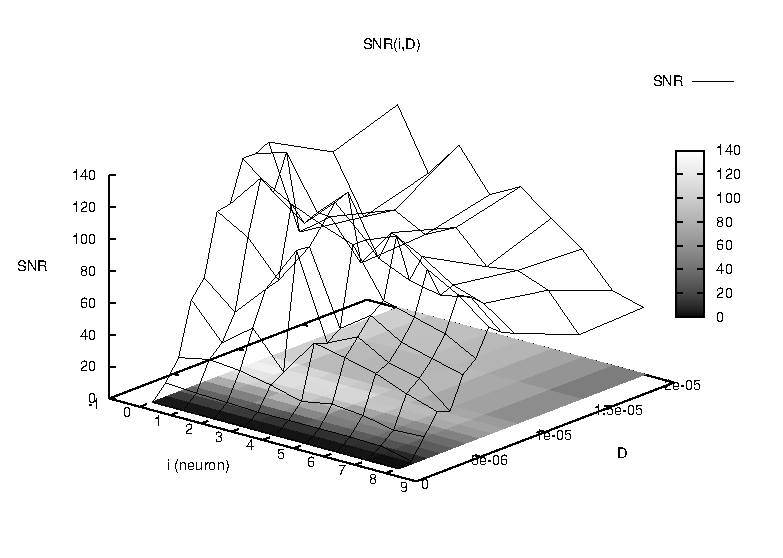
\includegraphics[width=140mm]{images/9neuron/2011_12_05_01}
    \caption{Układ 9 neuronów rozciągły przestrzennie o przesunięciu fazowym $\Delta \psi_{i,i+1} = 0.111 \cdot 2 \pi \cdot \zeta_{i,i+1}$ z opóźnieniem transmisji $c = 0.111 T$. 65536 ($2^{16}$) kroków iteracji (256 okresów). Pomimo pewnych różnic (niższy maksymalny SNR, wyższy SNR dla słabego szumu) widać wyraźne podobieństwo z wykresem na rys. \ref{fig:graphics:sim:2011_12_07_01}.}
    \label{fig:graphics:sim:2010_12_05_01}
  \end{figure}

  Wyniki tak zbudowanego układu przedstawia rysunek \ref{fig:graphics:sim:2010_12_05_01}.

  Zauważalne są różnice w przebiegu uśrednionych SNR. Maksymalne wartości SNR w układzie z niestałą rozciągłością są niższe, natomiast dla niskiego $D$ układ z niestałą rozciągłością ma zauważalnie wyższy SNR. Jednakże, pomimo obserwowalnych różnic, układ z opóźnieniem potrafi skompensować także pewne różnice w przesunięciu fazowym (oczywiście w pewnym, ograniczonym zakresie).

